Para iniciar o desenvolvimento de extensão do Bench4Q, iniciamos por trabalhar com uma versão completa da implementação do \textit{benchmark} Bench4Q \textbf{(adicionar link de download da ferramenta)}
----------------------------

Agora que a metodologia de extensão esta definida, apresenta-se um caso de estudo prático que demonstra como ela pode ser usada e aplicada para analisar o desempenho transiente de um sistema. Caso de estudo é uma metodologia ideal quando um holístico, investigação aprofundada é necessária %(Feagin, Orum, & Sjoberg, 1991). 

\section{O protocolo de caso de estudo}
Considere uma livraria que desejar realizar uma promoção no dia de seu aniversario, essa promoção é ousada e espera-se ter um grande volume de vendas decorre a comemoração, isso irá apoiar as suas operações de venda e expandir seu mercado. Logo, a maior preocupação por parte da empresa é que seu \textit{e-commerce} esteja disponível para os compradores/clientes, assim a empresa decidiu contratar os serviços de uma provedora de \textit{Cloud Computing} para hospedar o seu \textit{e-commerce} no dia o evento. O ambiente destinado para este evento está em processo de validação de carga, por parte da operadora, para garantir que os clientes antigos e novos da livraria possam usufruir e aproveitarem a promoção, e para a provedora não correr o risco de perderem o contrato o diretor de TI da provedora solicitou a sua equipe de engenheiros realizarem experimentos para garantir o desempenho esperado pelo cliente contrante.
Supondo que, em condições normais de funcionamento, o \textit{e-commerce} da livraria tem 10 clientes simultâneos e durante o dia do evento da mega promoção de aniversario, espera-se em média 20 clientes simultâneos,  além disso, a carga de trabalho está prevista para crescer em até 300\% ao longo do dia. A empresa contrante, a livraria, acredita que o tempo médio de resposta para todas as operações é de 7 segundos, e deseja que 90\% dos seus clientes estejam dentro dessas condições pré estabelecidas por ela, ou seja, a livraria da um margem de 10\% dos cliente fiquem fora do desempenho definido. Note-se que todos estes números e valores foram escolhidos de forma arbitrária, de modo a tornar o nosso cenário motivador mais específico.
Ao ler os requisitos de desempenho, a equipe de engenheiros, vez a necessidade de uma analise transiente, que por sua vez, buscam um \textit{becnhmark} para realizar os experimentos, então identificam um \textit{becnhmark} que se adéqua-se ao caso, entretanto o \textit{becnhmark} em questão não realiza analise transiente, contudo a equipe decide em aplicar a metodologia proposta neste trabalho.

Ainda assim, a equipe de engenheiro da operadora de \textit{Cloud Computing} precisa garantir e encontrar respostas para as seguintes perguntas, após a aplicação da metodologia:

\begin{itemize}
	\item Com a aplicação da metodologia, o \textit{becnhmark} irá estimular o sistema a apresentar a sua dinâmica, permitindo a analise em regime transiente do mesmo? 
	\item Que as métricas utilizadas pelo contratante são sendo analisadas
\end{itemize}

%Para um determinado número de servidores WebLogic, qual o nível de desempenho que o sistema fornece?

%Quantos servidores WebLogic seriam necessários para garantir o desempenho adequado sob a carga de trabalho esperada?

%Será que a capacidade do balanceador de carga e único servidor de banco de dados único suficiente para lidar com a carga de entrada?

%Será que a escala do sistema ou existem outros gargalos do sistema potencial?

%Vamos supor que o primeiro protótipo desta aplicação é SPECjAppServer2004 e que a empresa está testando a aplicação no ambiente de implantação mostrado na Figura 6.6. Este ambiente usa um cluster de servidores WebLogic (WLS) como um recipiente J2EE e um servidor de banco de dados Oracle (DBS) para persistência. Assumimos que todos os servidores no cluster WebLogic são idênticos e que, inicialmente, apenas dois servidores estão disponíveis.

%Com base nessas premissas, as seguintes metas concretas são estabelecidos:

%Prever o desempenho do sistema em condições normais de funcionamento com 4 e 6 servidores WebLogic, respectivamente. Qual seria o rendimento da transação média e tempo de resposta (para procurar, comprar e gerenciar)? Quantas trabalho ordens seria concluída por segundo no domínio de fabricação e qual seria o tempo médio de processamento da ordem de serviço? Como utilizada (CPU / utilização de disco) seriam os servidores WebLogic, o balanceador de carga eo servidor de banco de dados?

%?? Determinar se seis servidores WebLogic seria suficiente para garantir que os tempos médios de resposta de transações de negócios não exceda metade de um segundo durante condições de pico.

%?? Prever o quanto o desempenho do sistema poderia melhorar se o balanceador de carga é atualizado com um CPU um pouco mais rápido.

%?? Estudar a escalabilidade do sistema com o aumento da carga de trabalho e servidores WebLogic adicionais são adicionados.

%?? Determinar quais servidores seriam mais utilizados sob carga pesada e investigar se eles são potenciais pontos de estrangulamento. Em particular, verificar se a capacidade do balanceador de carga e único servidor de banco de dados único seria suficiente para lidar com a carga de entrada.


As seções a seguir mostram como estas questões podem ser respondidas por meio da metodologia de extensão proposto, além de uma apresentação detalhada do \textit{benchmark} que fora modificado pela metodologia.

%\subsection{Limitações do Bench4Q}

%Embora bastante sofisticado, o Bench4Q é primariamente um \emph{benchmark} para avaliação de desempenho em regime estacionário, uma vez que funciona a com base na pre-configuração da carga de trabalho \emph{off-line}.  A partir do início da simulação, a carga de trabalho é iniciada com as características estocásticas predeterminadas e permanece inalterada até o final do ensaio.  Não existem provisões para a introdução de perturbações controladas durante o processo, não propiciando facilidades para a exposição das propriedades dinâmicas da planta e registro dos efeitos transientes decorrentes de variações bruscas na carga --- o que é um ponto importante do sistema de controle proposto por  \citet{Nobile2013}.

\section{O \textit{Becnhmark}}

Sistemas de \textit{e-commerce} tem uma grande preocupação com os níveis de QoS, pois estão relacionados diretamente com os lucros do website. Atualmente a maioria dos \textit{e-commerce} são desenvolvido sensível a QoS. O Bench4Q é um \textit{benchmark} de um \textit{e-commerce} sensível a QoS.  Com o desenvolvimento da tecnologia Web, o TPC-W se tornou uma referência de \textit{e-commerce}, entretanto a implementação do TPC-W é insuficiente para \textit{e-commerce} sensíveis a QoS.

A maioria dos \textit{benchamarks} de \textit{e-commerce}, incluindo o TPC-W, são limitados para os sistemas sensíveis a QoS. As métricas utilizadas são baseadas em requisições HTTP, como a taxa de requisições atendidas com sucesso ou o tempo de resposta das requisições. Embora uma das características mais críticas de um sistema de \textit{e-commerce} sensíveis a QoS seja a integralidade do serviço prestado aos clientes, as métricas baseada em requisições podem levar a afinações ineficientes ou até mesmo erradas.


O Bench4q e é uma extensão do TPC-W (\textit{Transaction Processing Performance Council - Web})
\cite{Menasce2002}, O Bench4q tem como objetivo o \textit{tuning} de servidores \textit{e-commerce} orientados a fornecer QoS aos seus clientes. As principais características do Bench4Q incluem: 
apoio à análise de métricas baseada em sessão que simula carga sensível a QoS para uma análise da capacidade. 

O \textit{benchmark} Bench4Q, é distribuído de acordo com a \textit{GNU Lesser General Public License}, sendo um software livre ele pode ser redistribuído e/ou modificado sob os termos da licença publicas pela \textit{Free Software Foundation}. Seguindo muitas diretrizes da especificação TPC-W (\textit{Transaction Processing Performance Council - Web}), o Bench4Q usa principalmente nas suas métricas de simulação de carga e garantia de \textit{QoS} \cite{Bench4Q}. 

\textit{E-commerce}, que é uma loja virtual de comercio eletrônico, tem se tornado cada vez mais popular e ganhado cada vez mais concorrência com o desenvolvimento e expansão da Internet.vO Bench4Q é um \textit{benchmarking} que segue a metodologia de \textit{e-commerce} orientado a QoS, providos de recursos que permitem a simulação de um ambiente controlavel e flexível. Além disso, o Bench4Q pode ser usado para avaliar o desempenho de escalabilidade do sistema.

O trabalho \cite{cherkasova1998}, apresenta o conceito de sessão, que define uma sequencia de requisições de um único cliente. Krishnamurthy \cite{Krishnamurthy2006}, apresenta a dependência de sessões em sistemas \textit{e-commerce} e ressalta a importância de caracterizar a carga de trabalho sintética.

Apesar do grande sucesso do TPC-W, existe diversos trabalhos que apresentam métricas baseadas em sessões mais úteis do quais utilizadas pelo TPC-W. Ainda assim existe outro conjunto de trabalhos concentrado em como fazer TPC-W ser mais realístico. Em geral, essa obras tem inserido \textit{burstiness} na simulação de carga. O trabalho \cite{Mi2009} de Casale, incluiu o comportamento de \textit{burstiness}. Enquanto a obra \textbf{\cite{Sobel2008}}, busca adaptar o TPC-W para o ambiente em nuvem.

Embora a grande diversidade dos trabalhos apresentados, o Bench4Q oferece uma solução integrada para \textit{e-commerce} sensíveis a QoS. Vale salientar que, não há nenhuma solução integrada as características, especialmente, a de encontrar qualquer extensão TPC-W sensível a QoS para \textit{e-commerce}. Contudo, existem trabalhos que abordam a modelagem de rajadas no processo de chegada da carga de trabalho imposta ao sistema \textit{e-commerce}. Casale em \cite{Casale2012}, apresenta o BURN (\textit{BURtiness eNabling method}), uma metodologia para gerar rajadas customizáveis como demanda de carga de trabalho afim de avaliar o desempenho de um sistemas \textit{e-commerce}. A metodologia BURN é composta de duas políticas \textit{tradicional} (que gera a carga de trabalho constante a mesma gerada pelo TPC-W) e a \textit{burst} (que insere as rajadas na carga de trabalho tradicional). Durante a execução do \textit{benchmark}, BURN aplica um stress na aplicação \textit{e-commerce} alternando as duas politicas. Tais trabalhos buscam avaliar o desempenho sistemas de multi-camadas (composto por um servidor de aplicação, base de dados, etc) que hospedem um \textit{e-commerce} como é o caso do Bench4Q.

\subsection{Arquitetura}


O Bench4Q oferece uma arquitetura distribuída para a geração de carga através de seus agentes que são conectados a um único console que os gerencia, entretanto é possível configurar separadamente as configurações para cada agente. Esses agentes geram carga (requisições HTTP) para o servidor de aplicação onde esta hospedado o \textit{e-commerce} como ilustrado na figura \ref{fig:arquitetura-bench4q}. Os resultados da avaliação de carga aplicada ao \textit{e-commerce} são coletados pelo console que apresenta alguns gráficos, que facilita a interpretação da avaliação mediante as diretrizes do TPC-W que são complexas \cite{Bench4Q}.

A ferramenta é composta por três partes: Console, Agente e SUT-System Under Test, conforme apresenta a figura \ref{fig:arquitetura-bench4q}, e também disponibiliza interfaces para o monitoramento de recursos para o servidor de aplicação e para o banco de dados, este monitoramento incluem CPU, memória, rede, etc.

\begin{figure}[htb]
	\caption{Comportamento de métrica transiente}
	\label{fig:arquitetura-bench4q}
	\centering
	\includegraphics[scale=0.3]{bench4Q.png}
	\fdireta{Bench4Q}
\end{figure}

\begin{itemize}
	
	\item \textbf{Console:} A figura \ref{fig:console-bench4q} apresenta a interface do console, onde configura-se o teste, coleta e exibe os resultados. 
	
	\begin{figure}[htb]
		\caption{Console Bench4Q}
		\label{fig:console-bench4q}
		\centering
		\includegraphics[scale=0.5]{console-bench4Q.png}
		\fdireta{Bench4Q}	
	\end{figure}
	
	\item \textbf{Agente:} É este que faz o trabalho real, pois gera a carga configura no console. Simula o comportamento dos usuários no \textit{website}, disparando diversas requisições para o \textit{e-commerce}. 
	
	\item \textbf{SUT:} O \textit{e-commerce} SUT (\textit{System Under Test}), conforme apresentado na figura \ref{fig:sut},  é quem fornece o website de compras e está organizado com um banco de dados, servidor web e servidor de aplicativos. O portal compreende todos os componentes que fazem parte de uma aplicação real, isso inclui as conexões de rede, servidores web, servidores de aplicação, servidores de banco de dados, etc.
	
	\begin{figure}[htb]
		\caption{Bench4Q SUT}
		\label{fig:sut}
		\centering
		\includegraphics[scale=0.51]{sut.png}
		\fdireta{Bench4Q}
	\end{figure}
	
\end{itemize}


%\subsection{Bechmarks para computação em nuvem}
\subsection{Características do Bench4q}
\label{cap:caracteristicas-bench4q}
%\textcolor{blue}{
No contexto de sistemas de simulação, \textit{benchmark} é um software capaz de gerar carga de trabalho a ser aplicada a um sistema computacional com o objetivo de gerar dados acerca de uma métrica de forma que seja possível medir e comparar o desempenho de sistemas sob observação. Para os fabricantes de novos produtos, um \textit{benchmark} pode fornecer informações estatísticas importantes para que eles possam ser ajustados antes da sua implantação. Por outro lado, para os usuários finais, permite ter um ponto de referência na comparação entre pontos fortes e fracos de diferentes produtos. \textit{Benchmarks} ajudam em estimativas de escalabilidade em termos do número de usuários e/ou operações que um sistema pode suportar, e os tempos de resposta do sistema sob várias cargas e plataformas de implantação em hardware/software \cite{Jutla1999}.
%}

%edwin   
%\textcolor{blue}{
De uma maneira mais especifica, percebe-se que os \textit{benchmarks} para aplicações computacionais típicas de computação em nuvem, como \textit{e-commerce}, por exemplo, não são autalmente orientados a suportar totalmente QoS, porque alguns recursos de QoS críticos não podem avaliados por eles \cite{Zhang2011}. Um exemplo desses recursos é a integralidade do serviço, que é geralmente expressa como uma sessão fornecido aos clientes. Nesse sentido o Bench4Q tenta abranger essa lacuna.
%} 


O TPC-W (\textit{Transaction Processing Performance Council - Web} \footnote{TPC-W: \url{http://www.tpc.org/tpcw/}}), estendido pelo Bench4Q, é (mesmo atualmente tido como obsoleto) um \textit{ benchmark} direcionado a \textit{sites} de \textit{e-commerce} transacionais em que os consumidores são vinculados a sessões, cada cliente possui sua própria e única sessão em determinado instervalo de tempo. Trata-se de um site de venda de livros implementado em Java e hospedado em um servidor de aplicação Tomcat \footnote{Tomcat: \url{http://tomcat.apache.org/}}. Clientes (\textit{ browsers}) são emulados e se comportam como consumidores dos produtos oferecidos pela loja. Basicamente, os clientes podem interagir de diferentes formas: acessar a página inicial do \textit{ site}, navegar e procurar por produtos, realizar operações que envolvam o carrinho de compras e finalizar uma compra. A carga de trabalho gerada pelo TPC-W pode ser representada por um \textit{Customer Behavior Model Graph} --- CBMG, um grafo orientado, em que os nós representam uma operação a ser realizada (procurar, navegar, comprar etc.) e os pesos nas arestas significam a probabilidade de transição de uma operação para outra \cite{Zhang2011}. A Figura \ref{fig:CBMG} modela o fluxo de requisições a páginas e operações que um cliente pode realizar em uma sessão, basicamente um comportamento estocástico de acesso às páginas.

\begin{figure}[htb]
	\caption{CBMG - perfil interação estocástico}
	\label{fig:CBMG}
	\centering
	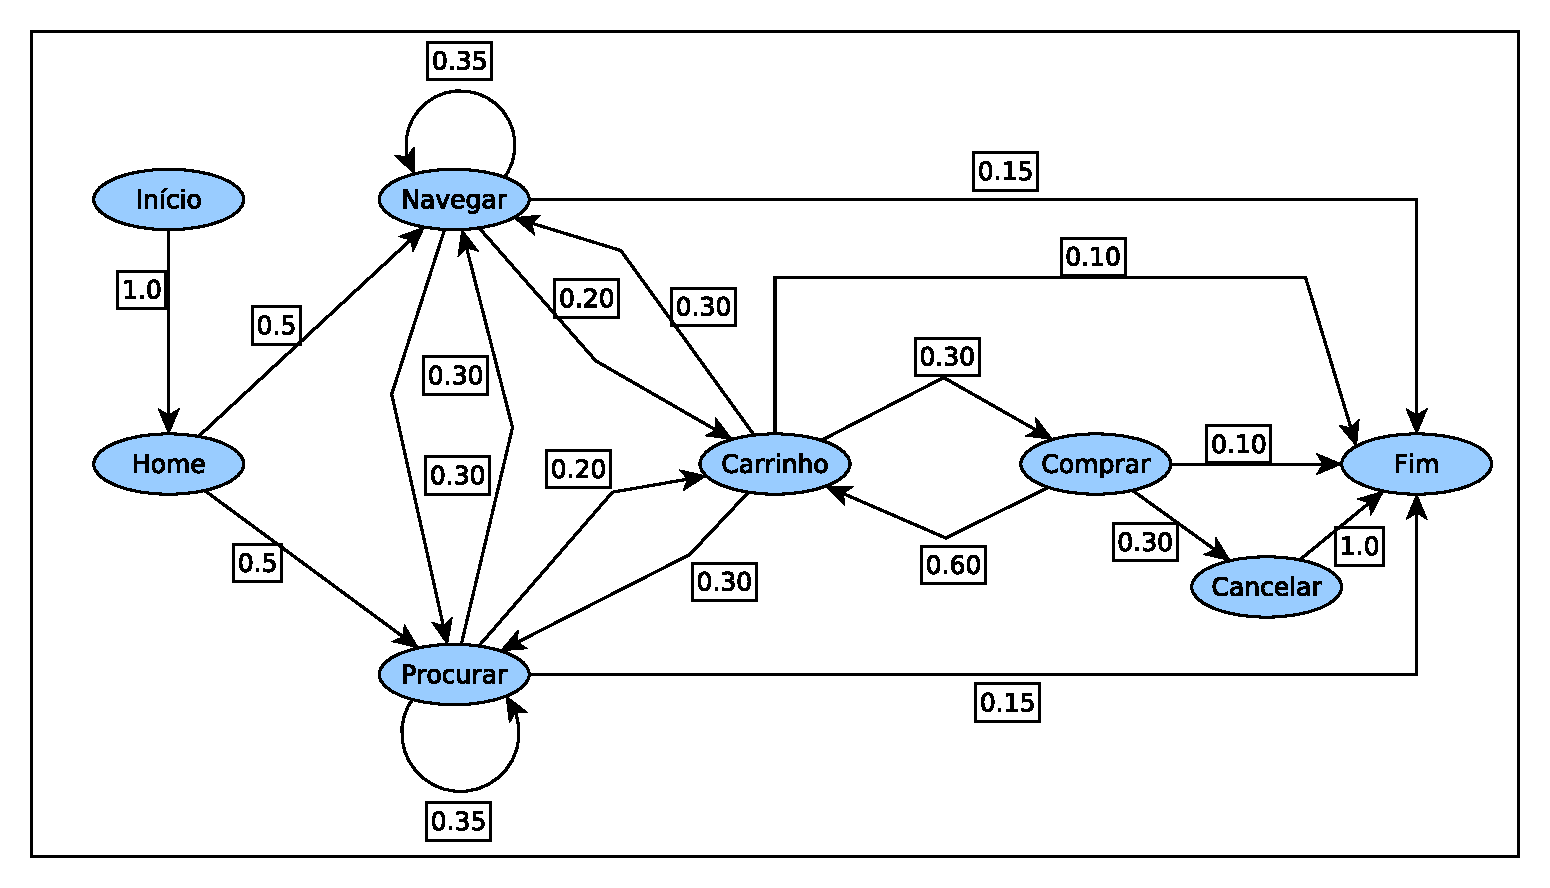
\includegraphics[scale=0.55]{CBMG.pdf}
	\fdireta{}
\end{figure}


A carga de trabalho gerada pelo TPC-W é formada por um CBMG com 14 tipos de interação \textit{web} e três perfis de pesos para suas arestas. O resultado é uma carga em que a maioria dos clientes apenas navega nas páginas (navegação: $95\%$ e compra: $5\%$); outra em que a maioria dos clientes realiza compras de forma moderada (navegação: $80\%$ e compra: $20\%$); e a terceira composta por muitos clientes que finalizam as compras (navegação: $50\%$ e compra: $50\%$). 

Vale ressaltar que existe um atraso entre as requisições de uma sessão. Ao iniciar uma sessão uma requisição é disparada e após receber a respectiva resposta, a próxima requisição acontece após um tempo também estocásticos e variante. Essa especificação tem o objetivo de emular melhor o comportamento humano ao acessar \textit{sites} de \textit{ e-commerce}.

Ao ser implantado em uma infraestrutura computacional que hospede todos seus componentes, os clientes emulados devem estar localizados fora de tal infraestrutura e conectados por uma rede. Os clientes começam as séries de requisições. O TPC-W implementa um modo de geração de carga conhecido como fechado (\textit{close mode}): um novo cliente chega somente após o antigo deixar o sistema \cite{Zhang2011}. As {\textbf métricas disponíveis} concernem basicamente sobre a quantidade de interações \textit{web}, sejam elas medidas em quantidade por segundo (\textit{ Web Interaction Per Second} --- WIPS) ou seu tempo de resposta (\textit{ Web Interaction Response Time} --- WIRT).

A motivação para a extenção do TPC-W e criação do Bench4Q começa porque, muito embora, as referidas métricas aparentem descrever bem a quantidade de acessos ao sistema, a qualidade do serviço experimentada pelo usuário pode ser desproporcional a essas mesmas métricas. Em \cite{bench4qslides} é descrito um ensaio que contempla dois cenários diferentes: um normal e outro otimizado não realisticamente. A otimização foi feita pela configuração de parâmetros no servidor Tomcat, a saber: {\texttt sessionTimeout}, {\texttt connectionTimeout} e {\texttt acceptCount}. Um das características da aplicação é a presença de operações \textit{ IO-bound}, por consequência, observar o tempo médio de resposta dessas operações permite diminuir os valores de estouro de tempo, e, com isso, forçar uma taxa de utilização de CPU. Assim, pode-se ``otimizar'' o ambiente da aplicação. Os resultados foram de $WIPS = 131$ para o cenário normal e $WIPS=199$ para aquele otimizado não realisticamente, corroborando com a hipótese. Porém, ao observar a quantidade de sessões completadas com sucesso (Figura \ref{fig:seeing}), percebe-se que o cenário normal permitiu uma quantidade de erros menor do que aquele otimizado não realisticamente. Por consequência, uma espectativa de lucro maior quando da implantação: maior quantidade de sessões realizadas sem error implicaria em maior probalidade de compras efetivas.

\begin{figure}[htb]
	\caption{Comparação da quantidade de requisições completadas com sucesso entre dois cenários: normal e otimizado não realisticamente.}
	\label{fig:seeing}
	\centering
	\includegraphics[scale=0.45]{seeing.png}
	\fdireta{Bench4Q}
\end{figure}


Tanto o TPC-W quando Bench4Q tem como objetivo produzir resultados que possibilitem o \textit{tuning} (sintonia do parâmetros) de servidores que compõem serviços de \textit{e-commerce} orientados a fornecer QoS aos seus clientes \cite{Menasce2002, Zhang2011}.  A ideia principal é que seja construída uma banca de testes (\textit{ testbed}), haja a execução do \textit{ benchmark} e consecutiva geração dos traços de execução, seja feita a extração dos dados e, por fim, com base nos resultados, melhores valores para os parâmetros de configuração do sistema sejam aplicados. Especificamente sobre o Bench4Q, as principais funcionalidade implementadas nele tem como contexto a observância do estado das sesões.
%}

%Neste capítulo será apresentado o \textit{benchmark} Bench4q que foi desenvolvido pelo \textit{Technology Center of Software Engineering} da \textit{Chinese Academy of Sciences} no \textit{Institute of Software}.
O \textit{ e-commerce} é um modelo de negócio bastante comum e possível principalmente por sua implantação em ambiente \textit{ web}, orientado a negociação de bens e serviços. Igualmente como o que acontece na forma tradicional de negociação, disputas por clientes e/ou fatias de mecardo surgem naturalmente, como podem ser observadas em promoções, ofertas, lançamentos de novos produtos etc. Portanto, um \textit{ website} alinhado a esses requisitos que proporcionem um desempenho melhor, ou seja, que possibilidade uma experiência melhor a seus usuários, certamente já começa melhor. Nesse sentido, o desempenho da infraestrutura que hospedará o negócio e o ajuste fino dos parâmetros operacionais da solução de \textit{ e-commerce} podem ser encarados como requisitos não-funcionais. Assim, seria possível realizar avaliações de desempenho que fomentem o projeto de tais sistemas cujo resultado sejam sistemas mais eficientes, mesmo que sejam abstraídas algumas regras específicas do negócio a ser implementado. O Bench4Q é uma ferramenta que possibilita tais projetos.
%\textit{E-commerce} (que é um \textit{website} com o proposito de vender bens como serviço) tem ganhado consideravelmente muitos adeptos a comercialização por este meio. Atualmente, existe uma competição entre \textit{e-commerces}, com promoções, ofertas e lançamento de novos produtos, assim como nas lojas físicas. O \textit{benchmark} Bench4Q, é uma ferramenta que disponibiliza uma estrutura de um comércio eletrônico para um ambiente controlável e flexível com a geração de carga de trabalho (baseada em sessão) que simula o comportamento autêntico de um usuário.

%\subsection{Características do Bench4q}

Sistemas de \textit{e-commerce} tem uma grande preocupação com os níveis de QoS, pois estão relacionados diretamente com os lucros do website. Atualmente a maioria dos \textit{e-commerce} são desenvolvido sensível a QoS. O Bench4Q é um \textit{benchmark} de um \textit{e-commerce} sensível a QoS.  Com o desenvolvimento da tecnologia Web, o TPC-W se tornou uma referência de \textit{e-commerce}, entretanto a implementação do TPC-W é insuficiente para \textit{e-commerce} sensíveis a QoS.

A maioria dos \textit{benchamarks} de \textit{e-commerce}, incluindo o TPC-W, são limitados para os sistemas sensíveis a QoS. As métricas utilizadas são baseadas em requisições HTTP, como a taxa de requisições atendidas com sucesso ou o tempo de resposta das requisições. Embora uma das características mais críticas de um sistema de \textit{e-commerce} sensíveis a QoS seja a integralidade do serviço prestado aos clientes, as métricas baseada em requisições podem levar a afinações ineficientes ou até mesmo erradas.


O Bench4q e é uma extensão do TPC-W (\textit{Transaction Processing Performance Council - Web})
\cite{Menasce2002}, O Bench4q tem como objetivo o \textit{tuning} de servidores \textit{e-commerce} orientados a fornecer QoS aos seus clientes. As principais características do Bench4Q incluem: 
apoio à análise de métricas baseada em sessão que simula carga sensível a QoS para uma análise da capacidade. 

O \textit{benchmark} Bench4Q, é distribuído de acordo com a \textit{GNU Lesser General Public License}, sendo um software livre ele pode ser redistribuído e/ou modificado sob os termos da licença publicas pela \textit{Free Software Foundation}. Seguindo muitas diretrizes da especificação TPC-W (\textit{Transaction Processing Performance Council - Web}), o Bench4Q usa principalmente nas suas métricas de simulação de carga e garantia de \textit{QoS} \cite{Bench4Q}. 

\textit{E-commerce}, que é uma loja virtual de comercio eletrônico, tem se tornado cada vez mais popular e ganhado cada vez mais concorrência com o desenvolvimento e expansão da Internet.vO Bench4Q é um \textit{benchmarking} que segue a metodologia de \textit{e-commerce} orientado a QoS, providos de recursos que permitem a simulação de um ambiente controlavel e flexível. Além disso, o Bench4Q pode ser usado para avaliar o desempenho de escalabilidade do sistema.

%\subsection{Capacidades, limitações e evoluções do Bench4q}

O trabalho \cite{cherkasova1998}, apresenta o conceito de sessão, que define uma sequencia de requisições de um único cliente. Krishnamurthy \cite{Krishnamurthy2006}, apresenta a dependência de sessões em sistemas \textit{e-commerce} e ressalta a importância de caracterizar a carga de trabalho sintética.

Apesar do grande sucesso do TPC-W, existe diversos trabalhos que apresentam métricas baseadas em sessões mais úteis do quais utilizadas pelo TPC-W. Ainda assim existe outro conjunto de trabalhos concentrado em como fazer TPC-W ser mais realístico. Em geral, essa obras tem inserido \textit{burstiness} na simulação de carga. O trabalho \cite{Mi2009} de Casale, incluiu o comportamento de \textit{burstiness}. Enquanto a obra \cite{Sobel2008}, busca adaptar o TPC-W para o ambiente em nuvem.

Embora a grande diversidade dos trabalhos apresentados, o Bench4Q oferece uma solução integrada para \textit{e-commerce} sensíveis a QoS. Vale salientar que, não há nenhuma solução integrada as características, especialmente, a de encontrar qualquer extensão TPC-W sensível a QoS para \textit{e-commerce}. Contudo, existem trabalhos que abordam a modelagem de rajadas no processo de chegada da carga de trabalho imposta ao sistema \textit{e-commerce}. Casale em \cite{Casale2012}, apresenta o BURN (\textit{BURtiness eNabling method}), uma metodologia para gerar rajadas customizáveis como demanda de carga de trabalho afim de avaliar o desempenho de um sistemas \textit{e-commerce}. A metodologia BURN é composta de duas políticas \textit{tradicional} (que gera a carga de trabalho constante a mesma gerada pelo TPC-W) e a \textit{burst} (que insere as rajadas na carga de trabalho tradicional). Durante a execução do \textit{benchmark}, BURN aplica um stress na aplicação \textit{e-commerce} alternando as duas politicas. Tais trabalhos buscam avaliar o desempenho sistemas de multi-camadas (composto por um servidor de aplicação, base de dados, etc) que hospedem um \textit{e-commerce} como é o caso do Bench4Q.

\subsection{Geração de carga}

A oscilação da carga de trabalho é uma característica fundamental. A simultaneidade dos acessos apresentam grandes efeitos sobre a escolha da política de ajuste de um servidor, o Bench4Q simular tal oscilação de carga atrás de seus agentes com os seguintes parâmetros:

\begin{itemize}
	\item \textit{Base Load:} Quantia fixa de \textit{threads} por agentes.
	\item \textit{Radom Load:} Quantidade de \textit{threads} que são geradas aleatoriamente.
	\item \textit{Rate:} O \textit{rate} (taxa de mudanças de carga), pode ser positivo, negativo ou nulo. Positivo significa que a carga de base está aumentando a cada segundo, se negativa significa que a carga de base está diminuindo a cada segundo e enquanto a taxa é zero, a carga é fixa.
	\item \textit{Trigger Time:} O tempo para o agente de carga para começar a gerar sua carga.
	\item \textit{Duration:} O tempo de execução do agente de carga.
\end{itemize}

As composições as cargas simuladas por diversos agentes, podem gerar as seguintes flutuações de carga típicas de empresas B2C podem ser simulados.

\begin{figure}[htb]
	\caption{Carga de trabalho gerada pelo Bench4Q}
	\label{fig:carga-gerada}
	\centering
	\includegraphics[scale=0.5]{load_fluctuation.png}
	\fdireta{Bench4Q}
\end{figure}


Existe dois modos de simulação de carga, o fechado e o aberto, conforme apresentado na figura \ref{fig:type-session}. No modo fechado, ilustrado na figura \ref{fig:type-session} (a), um novo cliente só acessará depois de cliente antigo deixar o sistema. Já o modo aberto, ilustrado na figura \ref{fig:type-session} (b), novos clientes vão acessar o sistemas sem se importa  com a saída dos antigos clientes. O TPC- W simula carga no modo fechado, o que faz uma suposição inexistente do mundo real \cite{Bench4Q}. 

\begin{figure}[htb]
	\caption{Tipo de sessões Bench4Q}
	\label{fig:type-session}
	\centering
	\includegraphics[scale=0.6]{type_session.png}
	\fdireta{Bench4Q}	
\end{figure}


Em sistemas baseados em sessões reais, como a proposta deste projeto, os clientes vêm com base em um modo aberto. Em sua utilização neste projeto, a sessão aberta é a que mais se adéqua a finalidade do objetivo proposto pelo trabalho.

\section{Implementação da metodologia}

Nesta seção é apresentado em detalhes a implementação dos passos da metodologia, proposta no capitulo \ref{chapter:metodologia}, e aplicadas no \textit{benchmark} Bench4Q.

\begin{figure}[htb]
	\caption{Diagrama de classe modificadas e adicionadas no Bench4Q.}
	\label{fig:diagrama-classes}
	\centering
	\includegraphics[scale=0.4]{diagrama-classes-beanch4Q.png}	
	%\fdireta{}
\end{figure}
	
%1º  - falar como foi implementados as modificações conforme a metodologia
Em primeiro lugar, e sem surpresa, e de acordo com a metodologia foi identificado o modulo de geração de carga do Bench4Q e este passou por alterações para gerar a carga de trabalho esperada. Conforme o diagrama de classes na figura \ref{fig:diagrama-classes}, é possível ter uma ideia do trabalho realizado no \textit{benchmark}, vale aqui salientar que o Bench4Q é uma ferramente completa e extensa, e diagramar todas as classes do mesmo ficaria difícil a sua apresentação em um único diagrama que facilita-se o entendimento, sendo assim, aqui apresentamos somente as classes já existente no Bench4Q e que passar por modificações para atender aos requisitos da metodologia e as novas classes que foram necessária para o mesmo objetivo.
%- montra diagrama de classes e diferenciando as classes existes com as que foram modificadas e adicionadas
 
	
Este conjunto de classes é que lida, manipula e gerencia a carga de trabalha gerada pelo Beanch4Q. A ferramente utiliza de um excelente console para configurar a carga de trabalho, e para mantar e respeitar o padrão do \textit{benchmark} foi implementado uma interface de configuração conforme ilustrado na figura \ref{fig:interface-criada-beanch4q}. Seguindo os padrões do Bench4Q, foi criado uma interface por onde controlar o comportamento da carga antes da execução, a carga é programada atras vezes de parâmetros informados previamente a execução do experimento. Exemplo, ao escolher a opção degrau, é necessário informar quantos EBs geram o degrau, em que instante de tempo, e qual o tempo de duração e por fim qual a sua polaridade (com base em um pulso elétrico a positiva sairia de zero e chega a um, a negativa, sairia de um e chegaria a zero).
%- mostrar a interface grafica de como ficou o Bench4Q

\begin{figure}[htb]
	\caption{Console de programação de carga de trabalho.}
	\label{fig:interface-criada-beanch4q}
	\centering
	\includegraphics[scale=0.5]{console-bench4Q-usp.png}
	%\fdireta{Console de programação de carga de trabalho.}
\end{figure}
	
	
%- mostrar resultados da carga de trabalho

%2º  - falar que nao foram necessarios incluir novas metricas, pois as presentes no bench4 já são o suficiente para o estudo de caso

O Segundo passo, de acordo com a metodologia apresentada, é a definição e coleta da métrica, esta por sua vez não foi implementada, pois as métricas propostas definidas nativamente pelo Bench4Q são relevantes conforme apresentado na seção \ref{cap:caracteristicas-bench4q}.

\section{Analise dos resultados}
%3º  - mostrar a analise e o impacto do carga de trabalho no sistema  
%Podemos agora usar os resultados da análise de desempenho para atender as metas estabelecidas no ponto 6.3.1. Por meio do modelo de QPN desenvolvido, que foram capazes de prever o desempenho do sistema em condições de funcionamento normais com 4 e 6 servidores WebLogic. Descobriu-se que usando o balanceador de carga original, seis nós de servidor de aplicação não foram suficientes para garantir tempos médios de resposta de transações de negócios abaixo de meio segundo. Atualizando o balanceador de carga com um CPU ligeiramente mais rápido levou à utilização de CPU do dropping balanceador de carga por um bom 20 por cento.
%Como resultado, os tempos de resposta de transações de concessionários melhorou em 15 a 27 por cento, encontrando o "meio segundo" exigência. No entanto, o aumento da intensidade da carga de trabalho além das condições de pico revelou que o balanceador de carga foi um recurso gargalo, impedindo-nos para escalar o sistema adicionando servidores WebLogic adicionais (veja a Figura 6.14). Assim, à luz do crescimento da carga de trabalho que o esperado, a empresa deve substituir a máquina balanceador de carga com um mais rápido ou considerar o uso de um método de balanceamento de carga mais eficiente. Depois de feito isso, a análise de desempenho deve ser repetida com o novo balanceador de carga para se certificar de que não há nenhum outro gargalos do sistema. Também deve ser assegurado que o balanceador de carga é configurado com threads suficientes para que não há contenção de discussão.
%Neste capítulo, a prática metodologia de modelagem de desempenho para DCS foi apresentada.
%A metodologia aproveita o poder de modelagem e expressividade do formalismo de modelagem QPN para melhorar a representatividade do modelo e permitir a previsão de desempenho precisas. Foi apresentado um estudo de caso detalhado no qual um modelo de um DCS realista foi construído e usado para analisar o seu desempenho e escalabilidade.
%O modelo de representatividade foi validado comparando suas previsões contra medições no sistema real. Foram considerados Um número de diferentes configurações de implantação e cenários de carga de trabalho. Além disso a CPU e I / O de contenção, demonstrou-se como alguns aspectos mais complexas do comportamento do sistema, tais como a contenção de rosca e processamento assíncrono, pode ser modelado. O modelo mostrou para refletir com precisão as características do sistema de desempenho e escalabilidade em estudo. O erro de modelagem para o tempo de resposta da transação não ultrapassou 21,2% e foi muito menor para a transferência de transações e utilização de recursos. A metodologia de modelagem de desempenho proposto fornece uma ferramenta poderosa para a engenharia de DCS desempenho.

1-Projete o protocolo de estudo de caso:
	a - determinar as competências necessárias
	b - desenvolver e revisar o protocolo

2-Conduta do estudo de caso:
	a - preparar-se para a coleta de dados
	b - distribuir questionário
	c - realizar entrevistas

3 Analisar caso provas estudo:
	a - analítica estratégia

4-Desenvolver conclusões, recomendações, e as implicações com base nas provas